\documentclass{article} % For LaTeX2e
\usepackage[final]{../colm2025_conference}

\usepackage{microtype}
\usepackage{hyperref}
\usepackage{url}
\usepackage{amsmath}
\usepackage{pifont}% http://ctan.org/pkg/pifont
\usepackage{booktabs}
\usepackage{soul}
\usepackage{cancel}
\usepackage{algorithm}
\usepackage{algpseudocode}
\usepackage{amsthm}
\usepackage{graphicx}
\usepackage{subfig}
\newtheorem{theorem}{Theorem}[section]

\usepackage{lineno}
\newcommand{\cmark}{\ding{51}}%
\newcommand{\xmark}{\ding{55}}%

\definecolor{darkblue}{rgb}{0, 0, 0.5}
\hypersetup{colorlinks=true, citecolor=darkblue, linkcolor=darkblue, urlcolor=darkblue}


\title{Weeks 3 \& 4: Implementing an RL Training Pipeline}

\author{\textbf{BEH} Chuen Yang}

\newcommand{\fix}{\marginpar{FIX}}
\newcommand{\new}{\marginpar{NEW}}

\begin{document}

\ifcolmsubmission
\linenumbers
\fi

\maketitle

\begin{abstract}
This document contains experiments on the CartPole-v0 Environment by \cite{Towers-et-al-2024}.
We compare the performance of a simple policy gradient (PG) algorithm and discuss
the viability of certain design choices in the training pipeline.
\end{abstract}

\section{Recap}
Refer to \cite{Levine-et-al-2023} and \cite{Week2} for a recap of the foundations of PG methods.
Essentially, PG algorithms optimize policies to maximize the expected return
via the following algorithm:

\begin{algorithm}[H]
    \caption{PG Algorithm}
    \label{alg:policy_gradient}
    \begin{algorithmic}[1]
        \State Input: Policy $\pi_\theta$, learning rate $\alpha$
        \State Output: Updated policy $\pi_\theta$
        \State Initialise policy parameters $\theta$
        \While{not converged}
            \State Sample a batch of trajectories $T$ from the policy $\pi_\theta$ and the environment
            \State Estimate the PG {\color{red} $\nabla_\theta J(\pi_\theta) \approx \frac{1}{m} \sum_{i=1}^{m} \left(\sum_{t=0}^{n} r(s_t, a_t)\right) \left( \sum_{t=0}^{n} \nabla_\theta \log(\pi_\theta(a_t | s_t)) \right)$}
            \State Update the policy parameters $\theta \leftarrow \theta + \alpha \nabla_\theta J(\pi_\theta)$
        \EndWhile
    \end{algorithmic}
\end{algorithm}

Notice however that this is not the only way to estimate the PG.
Particularly, we can switch out the PG estimation step (\textit{in red})
with more sophisticated gradient estimation rules in order to improve the stability and convergence of the algorithm.

\cite{Levine-et-al-2023} discuss several such improvements, and for brevity,
we will only write out the PG estimate for each improvement in isolation.
\begin{table}[h]
    \centering
    \begin{tabular}{p{0.225\textwidth} p{0.7\textwidth}}
        \toprule
        Improvement & PG Estimate \\
        \midrule
        Rewards To Go & 
        $\displaystyle \nabla_\theta J(\pi_\theta) \approx \frac{1}{m} \sum_{i=1}^{m} \left(\sum_{t={\color{red} k}}^{n} r(s_t, a_t)\right) \left( \sum_{t={\color{red} k}}^{n} \nabla_\theta \log(\pi_\theta(a_t | s_t)) \right)$ \newline
        where $k$ is the current timestep in the trajectory. \\
        \midrule
        Advantage Normalization & 
        $\displaystyle \nabla_\theta J(\pi_\theta) \approx \frac{1}{m} \sum_{i=1}^{m} \left(\sum_{t=0}^{n} {\color{red} A(s_t, a_t)} \right) \left( \sum_{t=0}^{n} \nabla_\theta \log(\pi_\theta(a_t | s_t)) \right)$ \newline
        where $A(s_t, a_t) = \frac{r(s_t, a_t) - \mu}{\sigma}$ is the advantage function. \\
        \midrule
        Reward Discounting & 
        $\displaystyle \nabla_\theta J(\pi_\theta) \approx \frac{1}{m} \sum_{i=1}^{m} \left(\sum_{t=0}^{n} {\color{red} \gamma^t} r(s_t, a_t)\right) \left( \sum_{t=0}^{n} \nabla_\theta \log(\pi_\theta(a_t | s_t)) \right)$ \newline
        where $\gamma < 1$ is the discount factor. \\
        \midrule
        Use of Baseline & 
        $\displaystyle \nabla_\theta J(\pi_\theta) \approx \frac{1}{m} \sum_{i=1}^{m} \left(\sum_{t=0}^{n} (r(s_t, a_t) {\color{red} - b(s_t)})\right) \left( \sum_{t=0}^{n} \nabla_\theta \log(\pi_\theta(a_t | s_t)) \right)$ \newline
        % This item had no explicit note in the original itemize structure
        \\ 
        \midrule
        Generalized Advantage Estimation (GAE) (\cite{Schulman-et-al-2018}) & 
        $\displaystyle \nabla_\theta J(\pi_\theta) \approx \frac{1}{m} \sum_{i=1}^{m} \left(\sum_{t={\color{red} k}}^{n} {\color{red} A(s_t, a_t)}\right) \left( \sum_{t={\color{red} k}}^{n} \nabla_\theta \log(\pi_\theta(a_t | s_t)) \right)$ \newline 
        where $k$ is the current timestep, $\gamma < 1$ is a discount factor, $A(s_t, a_t) = \sum_{l=k}^{\infty} (\gamma \lambda)^l \delta_{t + l}$, and $\delta_t = r(s_t, a_t) + \gamma V(s_{t + 1}) - V(s_t)$ is the temporal difference error. \\
        \bottomrule
    \end{tabular}
    \caption{Improvements to the PG Algorithm}
    \label{tab:pg_improvements}
\end{table}

Since \cite{Levine-et-al-2023} only consider a discount factor of $\gamma = 1$ (i.e. no discount) on a finite horizon task,
we will experiment empirically with only the first two improvements using a task due to \cite{Towers-et-al-2024}.

\section{CartPole-v0 Environment}
The CartPole-v0 environment by \cite{Towers-et-al-2024} is modelled after a classic reinforcement learning task 
by \cite{Barto-Sutton-Anderson-1983}, where the goal is to balance a pole on a cart by applying forces to the left or right. 

Table \ref{tab:cartpole_overview} summarizes the salient information about the environment.
\begin{table}
    \centering
    \begin{tabular}{ccc}
        \toprule
        Symbol & Description & Notes \\
        \\ \hline
        $s_t$ & $(x, v, \theta, \omega)$ & \begin{tabular}{c} $x$: Cart position \\ $v$: Cart velocity \\ $\theta$: Pole angle \\ $\omega$: Pole angular velocity\end{tabular}
        \\ \hline
        $s_0$ & $(x, v, \theta, \omega) \sim U(-0.05, 0.05)$ & 
        \\ \hline
        $a_t$ & [0, 1] & Left or Right.
        \\ \hline
        $r(s_t, a_t, s_{t + 1})$ & +1
        \\ \hline
        Termination & When pole "falls over", or $t \geq 200$
    \end{tabular}
    \caption{CartPole-v0 Environment Overview}
    \label{tab:cartpole_overview}
\end{table}

\section{Training Pipeline}
\subsection{Template Overview}

We were first provided with a template by \cite{Levine-et-al-2023} \textit{partially}
implementing a training pipeline for reinforcement learning (RL) algorithms.
The template includes a basic environment wrapper, a simple PG
algorithm, and a training loop that collects data from the environment and updates
the policy using the collected data.

\subsection{Implementation}
The template was missing most of the components 
for a theoretical PG algorithm.
\begin{itemize}
    \item Trajectory Collection: The template only partially defined the collection of a single trajectory.
    By extension, we cannot collect multiple trajectories.
    \item State-Value Estimation: The template did not calculate Q-values out-of-the-box.
    \item Advantage Estimation: The template did not calculate advantages out-of-the-box.
    \item Policy: While a network was built, the forward-pass and decision-making
    were not implemented.
    \item Update Loop: Loss Calculation and backpropagation were not implemented.
\end{itemize}

The specific changes made to the template have been detailed in the README
of the edited template, which can be found at \href{code/wk3/README.md}{code/wk3/README.md}.

\section{Experiments} 
In keeping with \cite{Levine-et-al-2023}, we ran the training pipeline on the \textit{CartPole-v0} environment
in order to study performance and convergence of the various PG algorithms
using Algorithm \ref{alg:policy_gradient} (and optionally, either rewards-to-go (RTG) 
or advantage normalization (AN) as in Table \ref{tab:pg_improvements}).

\begin{table}[h]
    \centering
    \begin{tabular}{ccc}
        \toprule
        Algorithm Variants & RTG & AN \\
        \midrule
        PG & \xmark & \xmark \\
        PG + RTG & \cmark & \xmark \\
        PG + AN & \xmark & \cmark \\
        PG + RTG and AN & \cmark & \cmark \\
        \bottomrule
    \end{tabular}
    \caption{PG Algorithms Tested}
    \label{tab:pg_algorithms}
\end{table}

For each algorithm variant, we ran trials with 10 different random seeds
and recorded the average train return over 200 sampling steps.
\begin{table}[h] \label{tab:hyperparameters}
    \centering
    \begin{tabular}{ccc}
        \toprule
        Hyperparameter & Value \\
        \midrule
        Trial Seeds & [941, 2370, 3295, 4495, 4943, 5653, 6548, 8497, 9127, 9540] \\
        Batch Size & {1000, 4000} \\
        Sampling Iterations & 200 \\
        \bottomrule
    \end{tabular}
    \caption{Hyperparameters for the Experiments}
    \label{tab:hyperparameters}
\end{table}

The training script for this experiment can be found at \href{code/wk3/train.py}{code/wk3/train.py}.

The average returns for each algorithm variant across \textit{ALL} seeds 
is shown in Figure \ref{fig:avg_returns}.
\begin{figure}[h]
    \centering
    \captionsetup{justification=centering}
    % \subfloat[Small Batch Size]{
    %     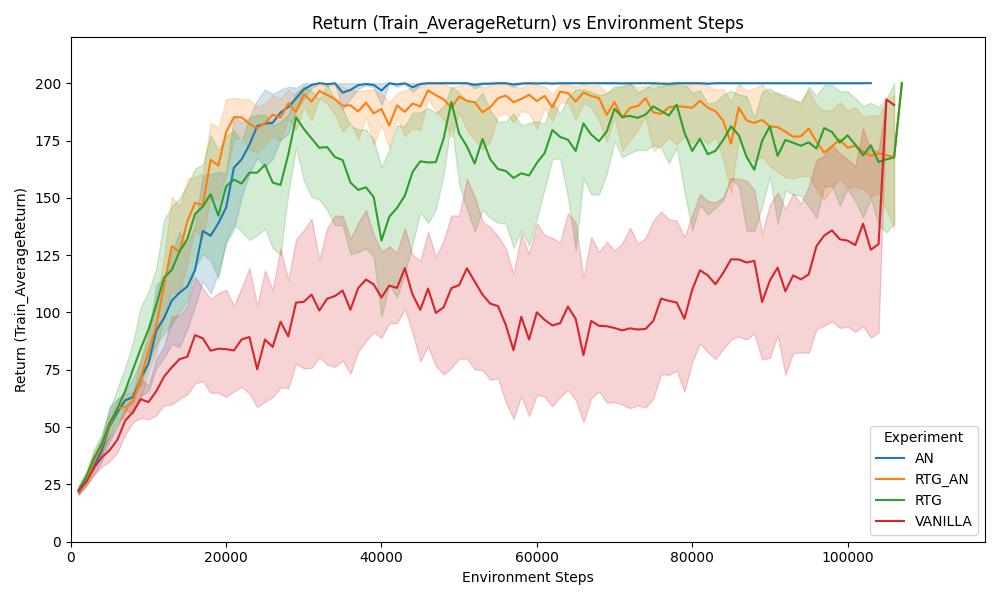
\includegraphics[scale = 0.8, width = 0.6\linewidth]{plots/return-vs-env-steps-small-batch.png}
    % }
    % \subfloat[Large Batch Size]{
    %     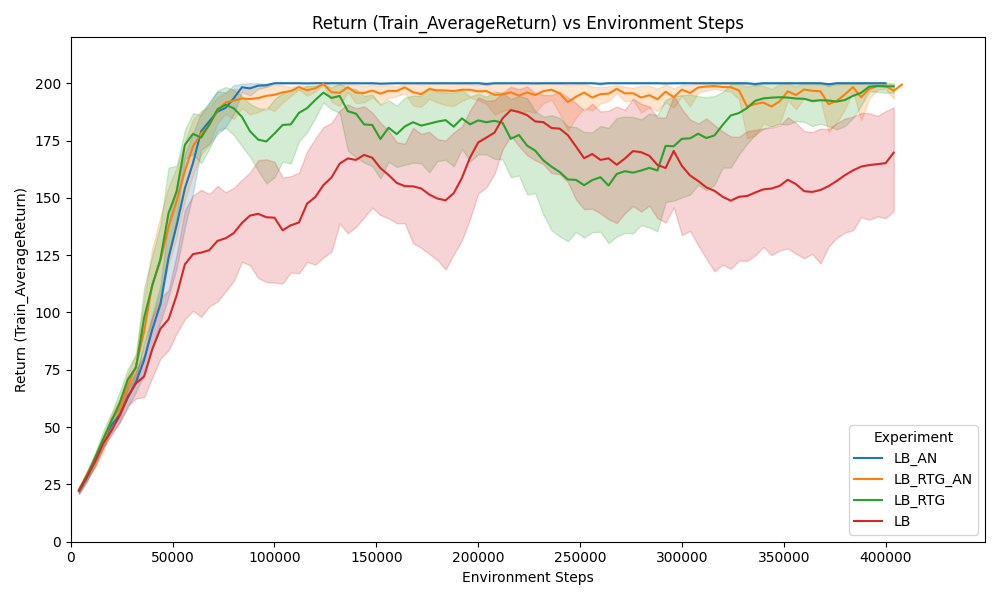
\includegraphics[scale = 0.8, width = 0.6\linewidth]{plots/return-vs-env-steps-large-batch.png}
    % }
    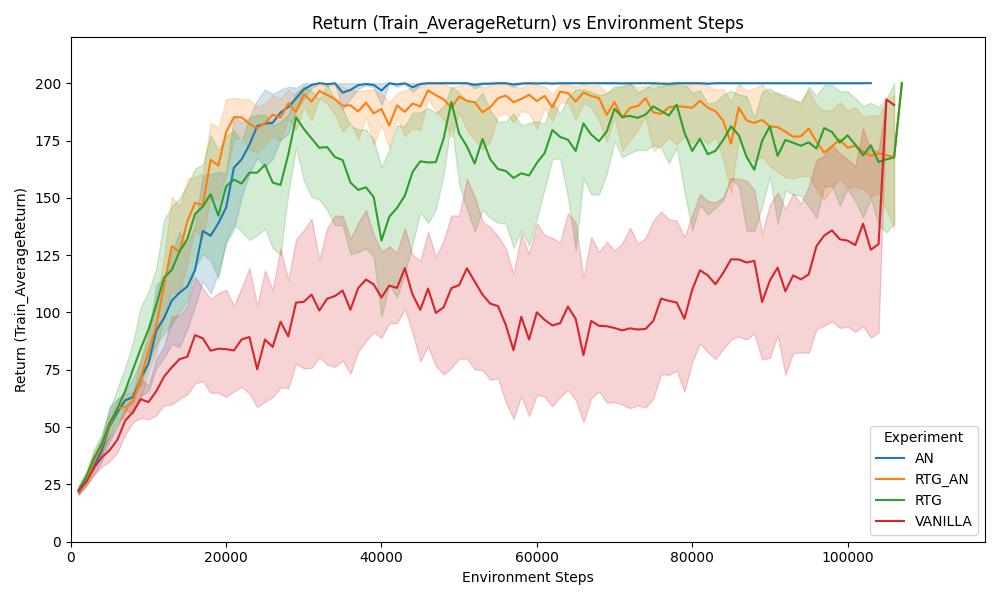
\includegraphics[scale = 0.6]{plots/return-vs-env-steps-small-batch.png}
    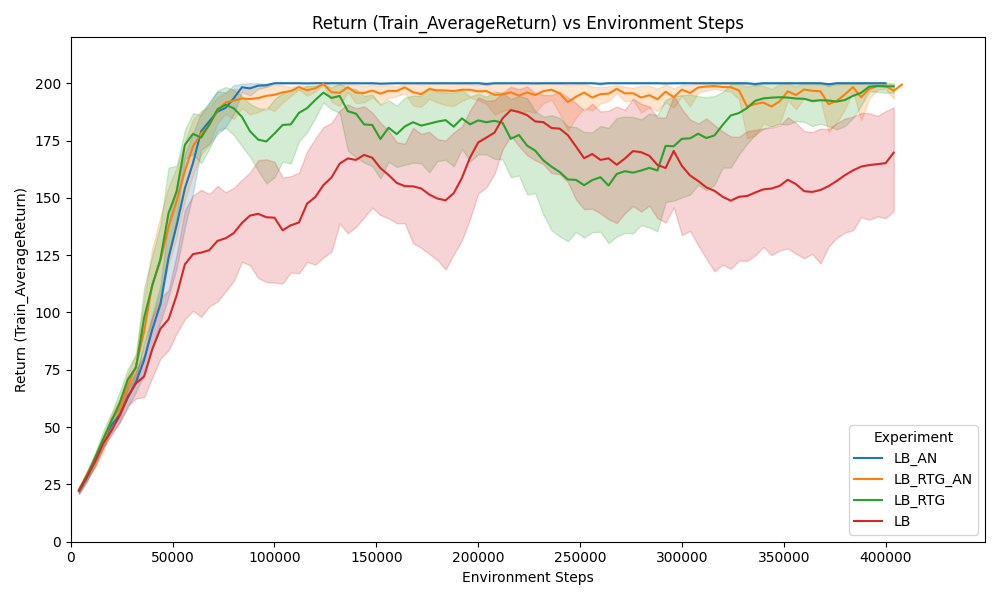
\includegraphics[scale = 0.6]{plots/return-vs-env-steps-large-batch.png}
    \caption{Average Returns for Each Algorithm Variant. For convenience of presentation, each datapoint was rounded to the nearest batchsize. \\ (Above) Small Batch Size (1000). (Below) Large Batch Size (4000).}
    \label{fig:avg_returns}
\end{figure}

\section{Discussion}
\subsection{Theoretical Expectations}
Due to the discussion of improvements to the PG algorithm in \cite{Levine-et-al-2023} and \cite{Week2},
we would expect the following trend:
\begin{itemize}
    \item PG should perform the worst, as it does not use any of the improvements.
    \item PG + RTG and PG + AN should perform better than PG since both techniques
    reduce variance in the gradient estimate, but we cannot say which will perform better.
    \item PG + RTG + AN performs the best, as it combines both improvements.
\end{itemize}

Moreover, by statistical intuition, we would expect the PG algorithm to work more reliably with a larger batch size,
which lends itself to more stable gradient estimates and hence a smoother learning curve.

\subsection{Empirical Results}
The empirical results in Figure \ref{fig:avg_returns}
\footnote{
    Detailed breakdowns of the performance of each algorithm variant
    across each individual seed and experiment type can be found in the appendices.
    See Appendices \ref{sec:experiment_type_plots} and \ref{sec:indiv_seed_plots} respectively.
} show that:
\begin{itemize}
    \item PG performs the worst, as expected.
    \item PG + RTG performs better than PG, but not as well as PG + AN, or PG + RTG + AN.
    \item Surprisingly, PG + AN performs better than PG + RTG + AN.
    \item A larger batch size leads to a smoother learning curve.
\end{itemize}

We offer some conjectures as to why this is the case in the following subsections.

\subsubsection{Impact of Advantage Normalization}
Advantage normalization (AN) predictably improves the performance of the PG algorithm.
By directly reducing the variance in the gradient estimate (through the advantage term),
the algorithm takes more stable steps in the direction of the gradient,
which \textit{CAN} lead to better convergence properties. 
\footnote{This is not necessarily the case. See \cite{Andrychowicz-et-al-2020} 
for data to the contrary.}

\subsubsection{Impact of Rewards-to-Go}
Likewise, the PG + RTG algorithm performs better than the PG algorithm,
and it is likely due to the fact that RTG reduces the variance in the gradient estimate,
as discussed in \cite{Levine-et-al-2023} and \cite{Week2}.

\subsubsection{Interplay of RTG and AN}
However, combining RTG and AN in the PG + RTG + AN algorithm yields a lower performance boost
than would be suggested by the sum of the individual improvements.

This is perhaps unique to our setup, which does not incorporate a value function baseline.
Specifically, we suspect that normalization of the RTG induces a bias towards earlier steps in the trajectory.

Since we are blindly averaging the returns \textit{from the current timestep onwards} across all steps in the trajectory, 
and our reward function is strictly non-negative on a per-timestep basis,
we neglect the fact that later timesteps are likelier to have lower returns as a result. 

Moreover, as the time dimension is not in the agent's state,
the agent does not learn why it receives lower returns at later timesteps.

Put together, this means that the agent will be unable to model the time-dependent aspects of the environment,
and will optimize for the earlier timesteps in the trajectory, which are more likely to have higher returns.
\footnote{
    This can be alleviated by including a time dimension in the agent's state.
    However, it appears that this is not common practice (at least, within \cite{Towers-et-al-2024}).
}
\footnote{
    A more permanent solution is to extend the environment into the infinite horizon case.
    This can be done by bootstrapping rewards with a value function,
    an approach best highlighted in temporal difference learning (TD-Learning),
    as exemplified in \cite{Sutton-1988}, and \cite{Schulman-et-al-2018}.
}

This causes the agent to learn a policy that is biased towards earlier timesteps,
which can lead to suboptimal performance.

\subsubsection{Impact of Batch Size}
As expected, a larger batch size leads to better performance as evidenced in Figure \ref{fig:avg_returns}.
Every experiment with a larger batch size, at least when we look at the percentage-wise progress of the average return,
has better expected return than the corresponding experiment with a smaller batch size.

Even considering the rewards on a per-timestep basis, the larger batch size experiments
have a higher expected return than the smaller batch size experiments, though the effect
is certainly less pronounced.

\subsection{Miscellaneous Observations}
In addition to the above observations, we also note a few points of interest when running the experiments:
\begin{itemize}
    \item From the wide confidence interval in Figure \ref{fig:avg_returns}, the \textit{PG algorithm appears very sensitive to the choice of random seed}, 
    perhaps due to the high variance in the gradient estimate.
    \item We occasionally observe \textit{extended periods of 
        performance degradation} (more obvious in Figure \ref{fig:returns_by_seed}), where the average return drops appreciably
        before recovering. 
        \begin{itemize}
            \item This is possibly due to \textit{catastrophic forgetting} (\cite{Goodfellow-et-al-2013}), which occurs as a consequence of the online nature of the algorithm,
            where collected data is always discarded after each update.
            \item Notably, since we can even see it in the averaged returns in Figure \ref{fig:avg_returns},
            this proves to be a relatively common occurrence.
        \end{itemize}
\end{itemize}

\section{Conclusion}
In this report, we have completed a training pipeline for a simple PG algorithm
and run experiments on the CartPole-v0 environment, with the goal of studying the performance 
of various tweaks to the simplest version of the PG algorithm. 

We have observed most significantly that the PG algorithm is sensitive to the choice of random seed,
that larger batch sizes can improve PG algorithms' performance, 
and that, at least without a baseline, advantage normalization (AN) is a more 
consistent and effective improvement than rewards-to-go (RTG). 
However, AN and RTG appear to synergize poorly.

\bibliographystyle{../colm2025_conference}
\bibliography{wk3}

\appendix
\section*{Appendix}
\section{Constant Hyperparameters}
In addition to the hyperparameters listed in Table \ref{tab:hyperparameters}, 
the following hyperparameters were kept constant throughout the experiments:

\begin{tabular}{ccc}
    \toprule
    Hyperparameter & Value \\
    \midrule
    $\alpha$ & 0.01 \\
    $\gamma$ & 1.0 \\
    Policy Network Architecture & 2 Linear layers with 64 units each, ReLU activation \\
    Optimizer & Adam \\
    Optimizer Betas & (0.9, 0.999) \\
    \bottomrule
\end{tabular}

\section{Experiment Type Plots} \label{sec:experiment_type_plots}
The following plots show the average return for each algorithm variant across each experiment type.
\begin{figure}[h]
    \centering
    \captionsetup{justification=centering}
    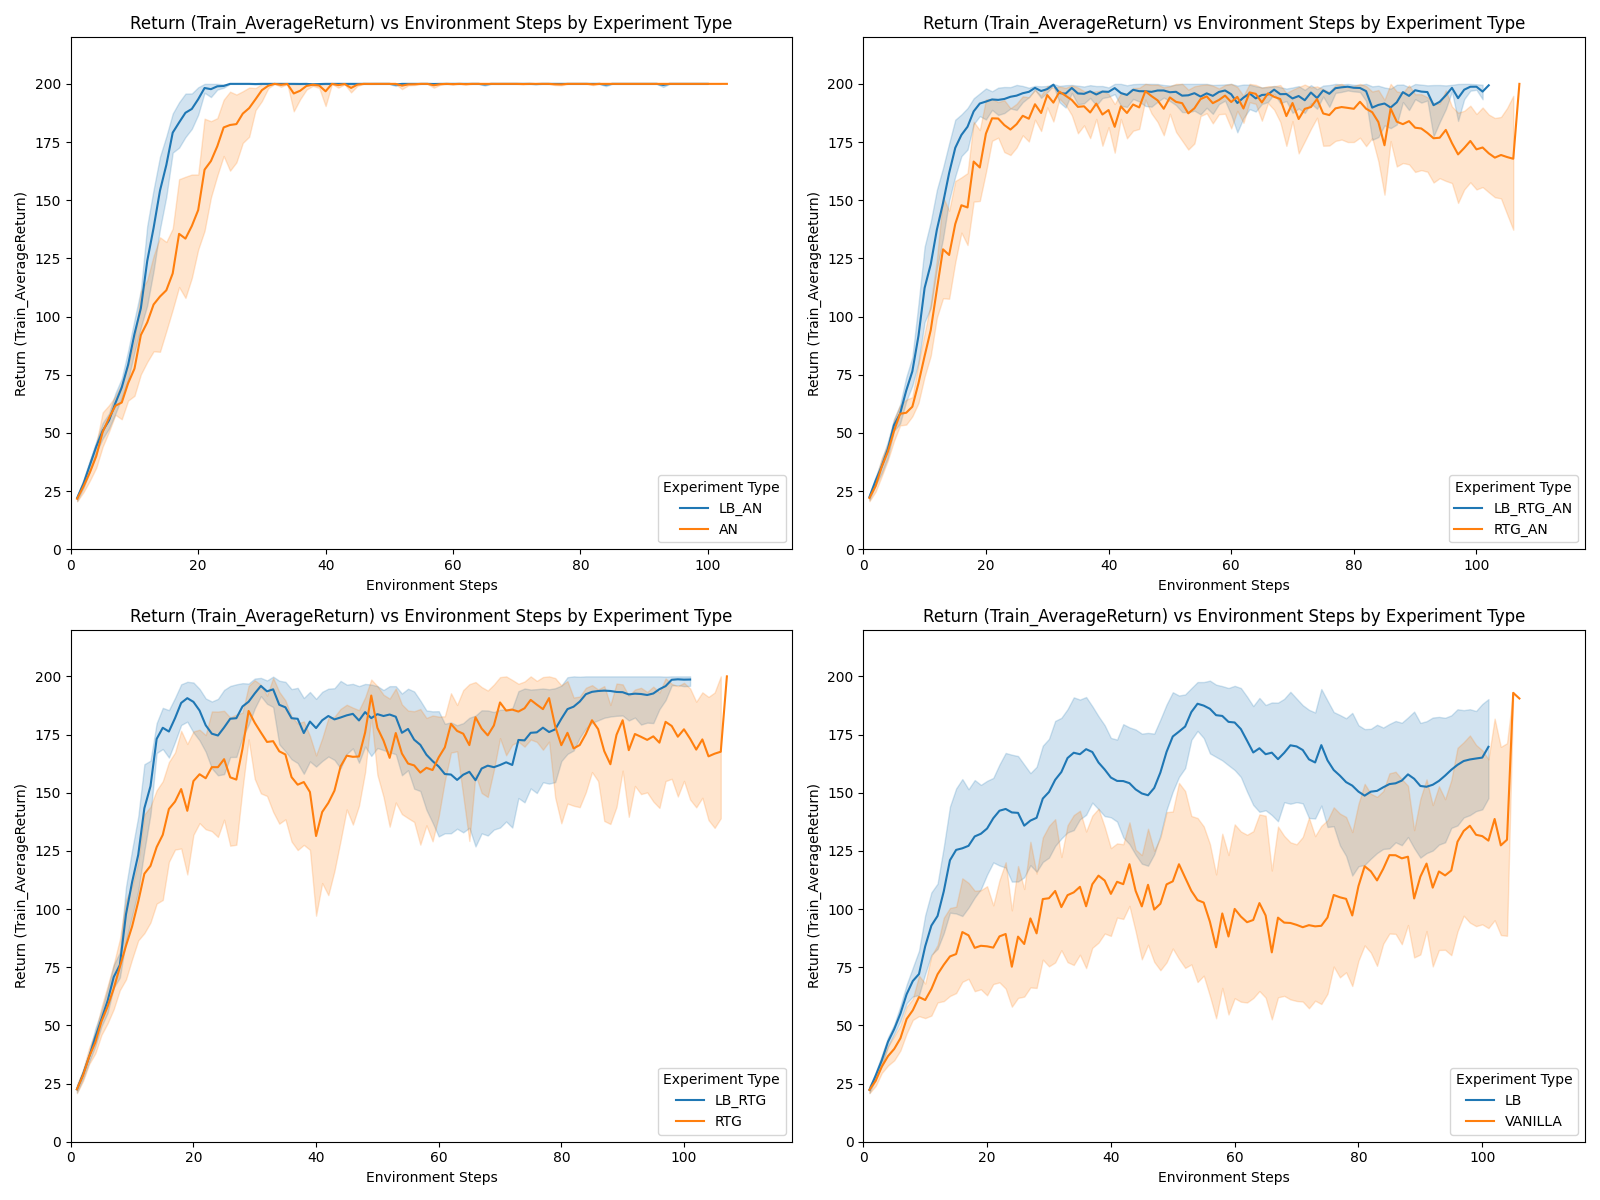
\includegraphics[width = \linewidth, height = 0.4\textheight]{plots/return-vs-env-steps-all-expt-types.png}
    \label{fig:returns_by_experiment_type}
    \caption{Returns for Each Algorithm Variant by Experiment Type. As with Figure \ref{fig:avg_returns},
    each datapoint was rounded to the nearest batch size for convenience of presentation.}
\end{figure}

\newpage
\section{Individual Seed Plots} \label{sec:indiv_seed_plots}
The following plots show the average return for each algorithm variant across individual seeds.
\begin{figure}[h]
    \centering
    \captionsetup{justification=centering}
    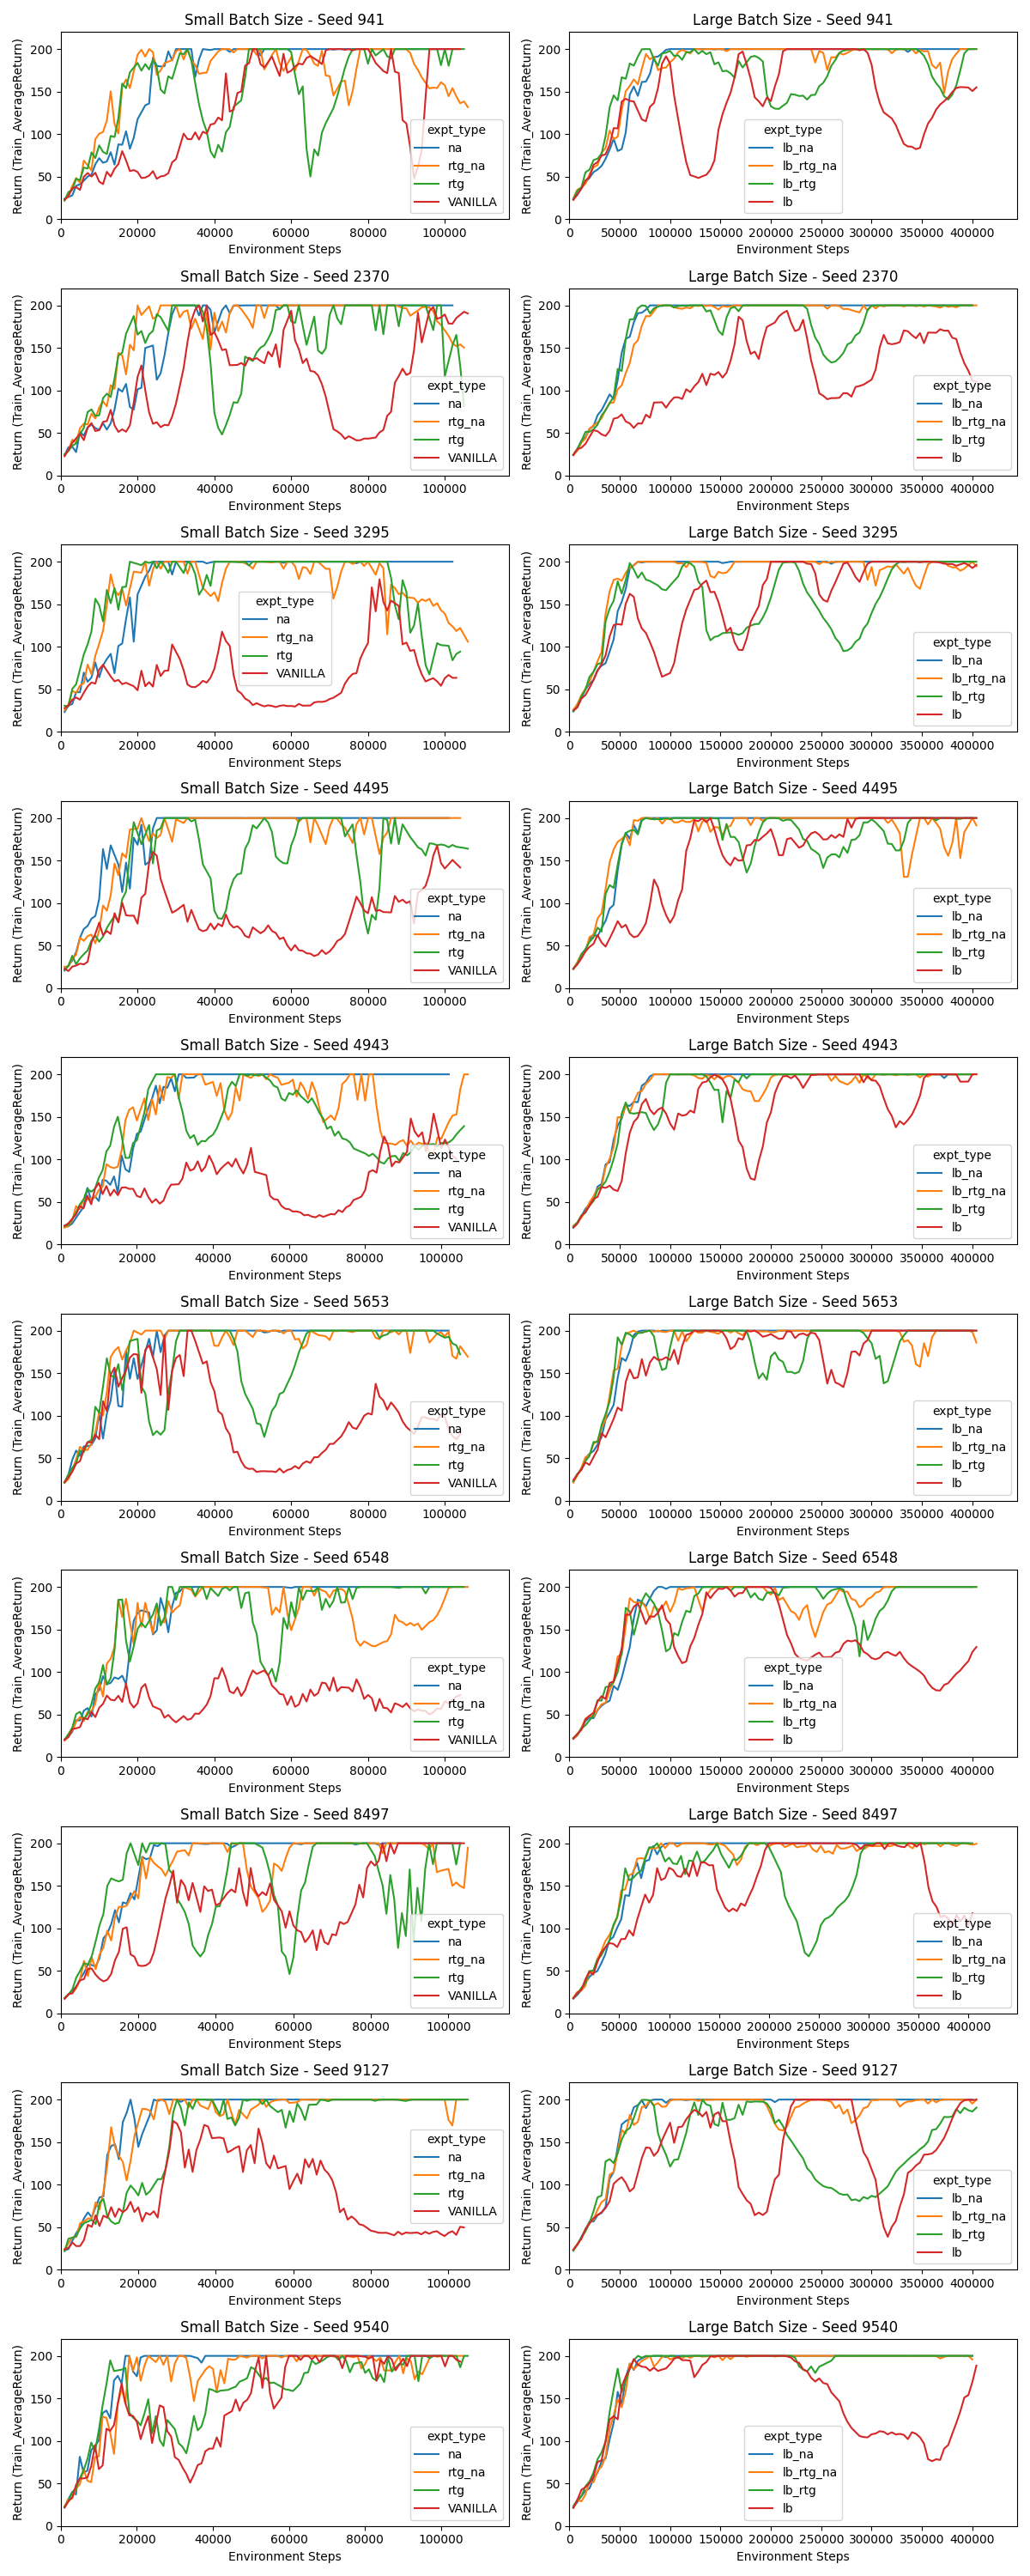
\includegraphics[width = \linewidth, height = 0.85\textheight]{plots/return-vs-env-steps-seeds.png}
    \caption{Returns for Each Algorithm Variant by Seed. As with Figure \ref{fig:avg_returns},
    each datapoint was rounded to the nearest batch size for convenience of presentation.}
    \label{fig:returns_by_seed}
\end{figure}

\end{document}